\chapter{Eliminación de palabras}
%El proceso de relacionar las palabras migrantes con campos semánticos y eventos históricos que justifiquen su aparición, permitió establecer un forma para cuantificar la influencia entre idiomas llamada uso. Todo este método se facilitó por la eliminación de las palabras funcionales, dejando sólo palabras de contenido, pero ¿cómo se modificaría el uso entre idiomas si se eliminaran otro tipo de palabras, sin importar si estás son de contenido?

%Para responder esta pregunta, se ha elaborado un nuevo algoritmo que reduce el conjunto de las palabras migrantes, y  obtiene nuevos valores para el uso entre idiomas.  Elegidos una pareja de idioma origen \textit{A} e idioma receptor \textit{B}, el proceso es el siguiente. 

En los métodos para cuantificar la influencia de un idioma en otro, ya sea a partir de las palabras nuevas o del uso que estas tienen en los diferentes receptores, se ha tratado de justificar los resultados con las palabras que intervienen en cada proceso. Sin embargo, dentro de las palabras migrantes, se encontraron errores al designar su idioma origen, errores que por el momento, no se sabe ni como eliminarlos ni como afectan a los resultados. 

El primer criterio que se hizo para minimizar errores y obtener mejores resultados, fue al eliminar las palabras funcionales, dejando sólo las palabras de contenido. Este criterio disminuyó la cantidad de palabras migrantes, por lo que es comprensible pensar que tras una limpieza en los resultados, la cantidad de ellos se reducirá. 

Con la idea anterior, al no tener otro tipo de criterios para limpiar los datos, se pueden simular reglas que reduzcan la cantidad de palabras migrantes. Una vez hecha la reducción, se puede obtener el uso de un idioma en otro para compararlo con los resultados previos. Se decidió comparar con el uso y no con las palabras nuevas, ya que en cada año hay más prestamos acumulados que préstamos nuevos (en algunos años no hay palabras nuevas), además la intención de las posibles reglas, es reducir el tamaño de los conjuntos no desaparecerlos.

El proceso para simular reglas y hacer las eliminación es el siguiente. 

\begin{enumerate}
	
	\item Se toma la lista de los préstamos acumulados de \textit{A} en \textit{B},  este corpus se denotará como \textbf{conjunto original}.
	
	\item Se escogen de forma aleatoria un grupo de letras (desde una hasta diez), y se descartan del conjunto original a aquellas  palabras cuya primer letra sea alguna de las elegidas. El nuevo corpus se denotará como \textbf{conjunto reducido}.
	
	%\item Se designa un tercer corpus como \textbf{conjunto residuo}, conformado por todas las palabras eliminadas del conjunto original.  La unión del reducido con el residuo es el original. 
	
	\item En los dos conjuntos se emplea la ecuación \ref{ec.fuso} para encontrar el uso de \textit{A} en \textit{B}.
	
	
\end{enumerate}

%La intención de este método  no es eliminar a todas las palabras migrantes, sino el reducirlas  para  comparar el uso entre el conjunto original y el reducido.  Para determinar que tanto ha cambiado el uso en los dos conjuntos, se utilizará el coeficiente de determinación $R^{2}$. 

%El primer criterio será al tomar el uso en el conjunto original como verdadero (ya que con el se establecieron los resultados del capítulo anterior), donde sus valores para un tiempo $t$ se expresan como $O_{t}$. Si en el conjunto reducido   es el uso para el mismo $t$, mientras que  $\bar{v}$ es el promedio de todos los valores de uso, entonces  el coeficiente de determinación queda definido como:

Si el uso en el conjunto original se toma como verdadero (ya que con el se obtuvieron los resultados del capítulo anterior), una forma de determinar que tanto cambió el uso en el conjunto reducido, es a partir del coeficiente de determinación $R^{2}$. 

%Si para un año $t$ dentro de un intervalo de tiempo $\Delta t$,  se detonan como $O_{t}$ al uso en el conjunto original y $v_{t}$ al uso en el al uso en el conjunto reducido,  mientras que $\bar{v}$ es el promedio de todos los $v_{t}$ en el intervalo, entonces el coeficiente de determinación se expresa como: 
Para un año $t$ dentro de un intervalo de tiempo $\Delta t$,  el uso en el  conjunto original y el uso en el conjunto reducido se detonan como $O_{t}$ y $v_{t}$ respectivamente,  mientras que $\bar{v}$ es el promedio de todos los $v_{t}$ en el intervalo, entonces el coeficiente de determinación queda definido como: 
\begin{equation}
\label{ec.dif_uso}
R^{2} = 1 - \sum_{t} \frac{ \left( v_{t}- O_{t} \right)^{2}  }{ \left( v_{t} - \bar{v} \right)^{2} }.
\end{equation}
Se empleará el concepto \textbf{conservación del uso} para aquellos idiomas cuyo uso no cambie en un intervalo de tiempo. La conservación es favorable si $R^{2}$ es próximo a 1. 
%Si la conservación no es favorable, las palabras eliminadas son las más relevantes para las migraciones de \textit{A} en \textit{B}.

\section{Características de las eliminaciones}


El procedimiento de eliminar palabras, obteniendo el uso y el coeficiente de determinación, se realizó cien mil veces, cinco mil por cada pareja de idiomas. Tras las eliminaciones, se graficaron algunos casos obtenidos, representando con un trazo continuo al uso en el conjunto original, mientras que el uso en el conjunto reducido es una serie de puntos; en cada grafica se especifican las letra con las que se hicieron la eliminaciones. 

Después de analizar las graficas de cada pareja de idiomas, se concluyó  que el uso en ambos conjuntos, cumple alguna de las siguientes características.


\begin{itemize}
	
	\item Valores iguales. Punto a punto, el uso en ambos conjuntos es el mismo. En este caso, el uso se conserva ya que las graficas son indistinguibles (figura~\ref{fig.OM1}).
	
	\item Diferencia de altura. En la mayor parte de los puntos, existe una diferencia casi constante entre ambos valores de uso. En este caso, el uso también se conserva, ya que las graficas son iguales sólo que están desplazadas (figura~\ref{fig.OM2}).  
	
	\item Alteraciones por periodos. El uso de ambos conjuntos,  en algún intervalo de tiempo, es completamente diferente. En este caso, el uso no se conserva, ya que la graficas son diferentes (figura~\ref{fig.OM3}).

\end{itemize}



%Para ilustrar las caracterizaras mencionadas, se exponen algunas graficas obtenidas, representado con un trazo continuo al uso del conjunto original, mientras que el uso en el conjunto reducido  es una serie de puntos.  Ya que los valores en el conjunto residuo son muy pequeños, se opto por no graficarlos, para no saturar la información. 

%En cada grafica se especifican los idiomas que intervienen, así como el conjunto de letras con las cuales se hicieron las eliminaciones. 



\begin{figure}[h!]
	\centering
	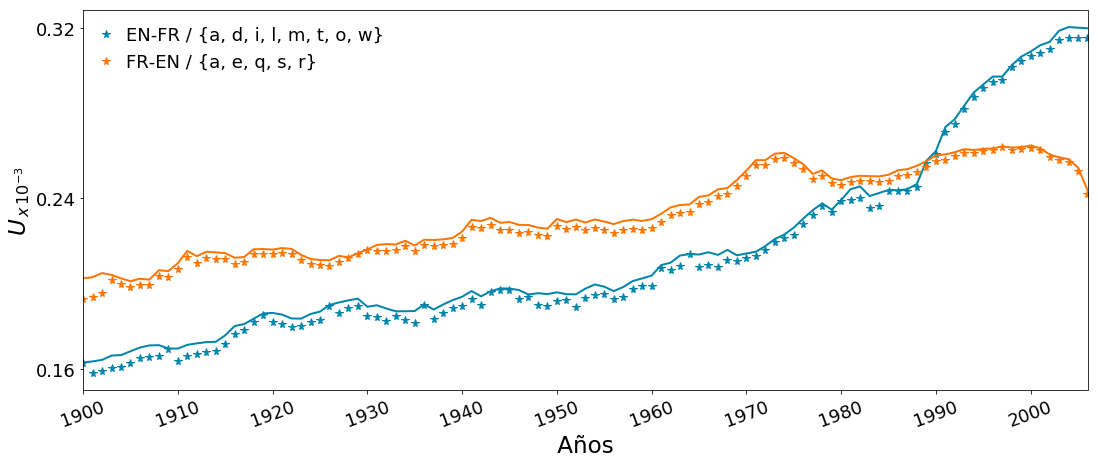
\includegraphics[scale=.375]{OM1.png}
	\caption{Eliminación de palabras en el inglés y en el francés. El uso se conserva en ambas parejas de idiomas durante todo el siglo XX, ya que $R^{2}$=0.99 para el inglés-francés y $R^{2}$=0.95 para el francés-inglés.}
	\label{fig.OM1}
\end{figure}


\begin{figure}[h!]
	\centering
	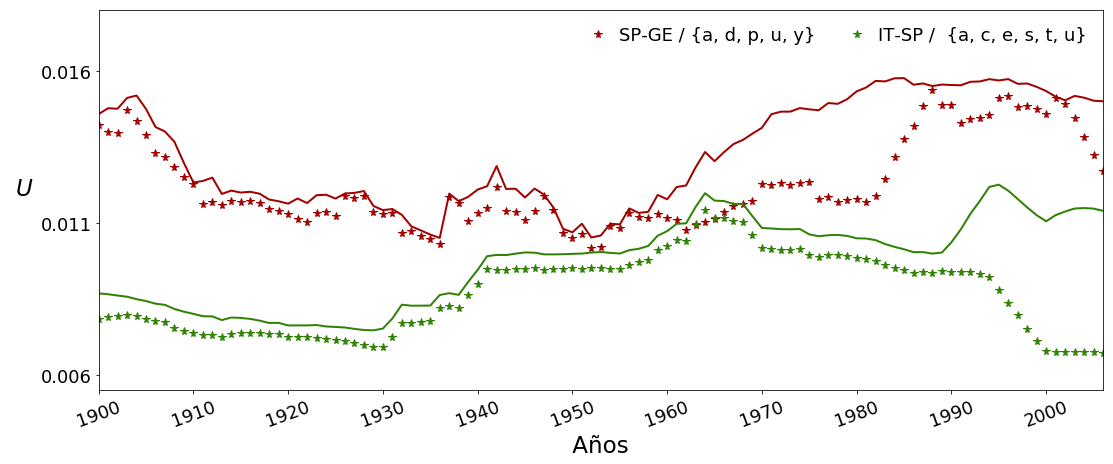
\includegraphics[scale=.375]{OM2.png}
	\caption{Eliminación de palabras en el alemán y en el italiano. El uso se conserva en ambas parejas de idiomas durante todo el siglo XX, existiendo una diferencia de altura entre el uso original y el uso reducido.  Al despreciar la diferencia, $R^{2}$=0.86 para el alemán-inglés y $R^{2}$=0.82 para el italiano-francés.}
	\label{fig.OM2}
\end{figure}

\begin{figure}[h!]
	\centering
	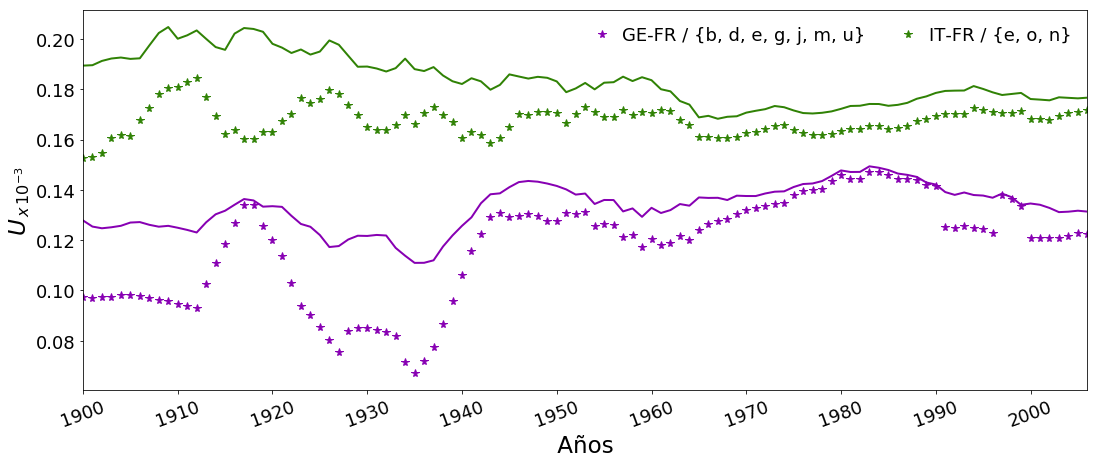
\includegraphics[scale=.375]{OM3.png}
	\caption{Eliminación de palabras en el español. Entre 1955 y 1985 el uso del español-alemán no se conservo, correspondiendo un valor de $R^{2}$=0.16 entre esos años.}
	\label{fig.OM3}
\end{figure}


La conservación del uso y sus características no siempre serán la mismas tras una eliminación con diferentes letras, sin embargo, es posible decir 
con los datos de las cien mil eliminaciones, si el uso se conserva.  Para ello, se agruparon y promediaron por cada idioma origen  los valores del coeficiente de determinación, obteniendo un $\left \langle R^{2}  \right \rangle$  promedio con el cual decir de manera general, si el uso del idioma origen se conserva. 

La tabla~\ref{tab.conservacion} muestra por cada idioma origen,  el valor de $\left \langle R^{2}  \right \rangle$ correspondiente, así como  en cuales idiomas receptores el promedio de $R^{2}$ fue mayor, y en cuales el promedio $R^{2}$ fue menor. De esta tabla se puede ver que el alemán es el idioma con los valores más bajos de $R^{2}$, donde la menor conservación se dio con el español. Los demás idiomas tienen valores aceptables con los cuales decir que su uso se conserva a pesar de las eliminaciones. 

Como la intención de las eliminaciones es simular reglas que limpien los datos, se puede decir que los préstamos con más errores son los del alemán en el español, ya que si se hubiese tal criterio, los resultados de esta pareja serian los más afectados. En los demás idiomas no habría un cambio significativo. 


 
%De esta tabla se puede ver que la conservación del uso es menor, en las combinaciones donde el alemán este presente, ya sea como idioma origen o como idioma receptor. No obstante, en los demás idiomas la conservación del uso fue favorable, por lo que se puede decir que los idiomas conservan su uso, sin importar  cuales sean las palabras que conformen a las migraciones. 


 

%Con estos resultados se puede decir que el uso entre idiomas, no es afectado por reducir la cantidad de palabras que conforman a las migraciones,   


\begin{table}
	\centering
	\begin{tabular}{cccc}
		\textbf{} & \textbf{$\left \langle R^{2} \right \rangle$} & \textbf{$R^{2}_{max}$} & \textbf{$R^{2}_{min}$} \\
		\textbf{inglés}   & 0.85 $\pm$ 0.14   &  IT 0.97 $\pm$ 0.01  & GE 0.77 $\pm$ 0.03  \\
		\textbf{francés}  & 0.83 $\pm$ 0.12   &  EN 0.95 $\pm$ 0.02  & GE 0.66 $\pm$ 0.02  \\
		\textbf{alemán}   & 0.75 $\pm$ 0.06   &  EN 0.80 $\pm$ 0.06  & SP 0.51 $\pm$ 0.33  \\
		\textbf{italiano} & 0.87 $\pm$ 0.14   &  FR 0.93 $\pm$ 0.08  & GE 0.68 $\pm$ 0.03  \\
		\textbf{español}  & 0.88 $\pm$ 0.05   &  IT 0.94 $\pm$ 0.06  & GE 0.71 $\pm$ 0.01                                                               
	\end{tabular}
	\caption{Conservación del uso de los idiomas. El español es el idioma que es menos afectado por las eliminaciones y que conserva más su uso en los demás, seguido del italiano, el inglés, el francés y por ultimo el alemán.}
	\label{tab.conservacion}
\end{table}





\section{Resultados generales}

El realizar diferentes elecciones para reducir la cantidad de palabras migrantes, mostró que los posibles errores en la clasificación de los datos, no modifican (en la mayoría de los casos) los resultados obtenidos. 

También se destaca al uso de un idioma en otro, como una propiedad común para cada pareja de idiomas, donde no tiene relevancia la cantidad  de palabras que conformen los préstamos acumulados,  en conjunto, todas ellas se comportarán de la misma manera. 



%El tratar a las migraciones de palabras como un conjunto, donde no tiene tanta relevancia las palabras que lo conforman, muestra propiedades estadísticas comunes que cumplen las parejas de idiomas. Por el momento  

   




%Individualmente. los valores de uso de una única palabra pueden ser distintos a los de otra palabra, sin embargo al tratar a todo el conjunto, el uso se comporta de la misma manera, sin importar los valores individuales de los elementos que lo conforman. 

%A pesar de haber errores en el algoritmo que clasifica tanto a los idiomas orígenes, como a sus  palabras migrantes, la conservacion del uso puede justificar que no importa si se eliminan las palabras mal clasificadas, en términos numéricos, el uso de un idioma otro va a ser el mismo.  

